
\documentclass[12pt,a4paper]{article}
\usepackage{amsmath,amssymb}
\usepackage{tikz}
\usepackage{pgfplots}
\usepackage[margin=1in]{geometry}
\usepackage{CJKutf8}
\begin{document}
\begin{CJK}{UTF8}{min}

\section*{問題}
次の二次関数 $f(x) = x^2 - 4x + 3$ と直線 $g(x) = 2x - 1$ のグラフの交点を求めよ。

\begin{center}
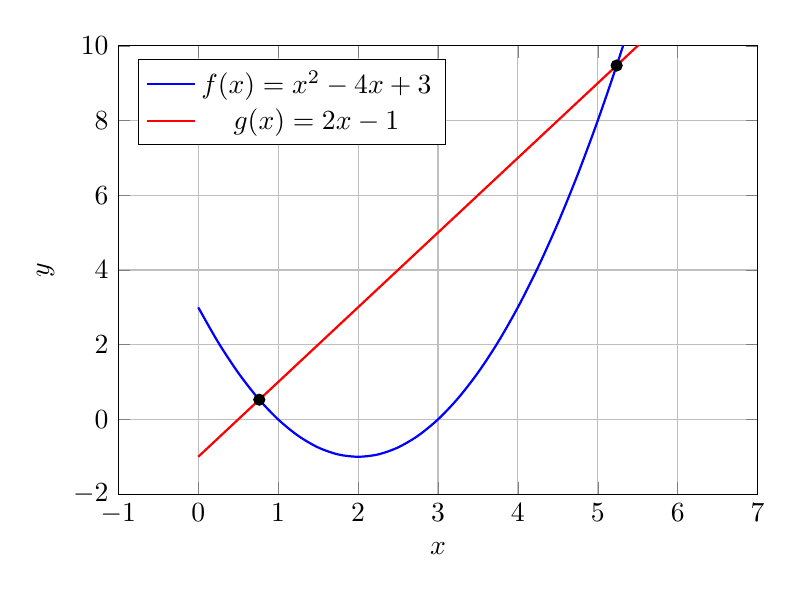
\begin{tikzpicture}
\begin{axis}[
  xlabel={$x$},
  ylabel={$y$},
  xmin=-1, xmax=7,
  ymin=-2, ymax=10,
  grid=both,
  minor grid style={gray!25},
  major grid style={gray!50},
  width=0.8\textwidth,
  height=0.6\textwidth,
  legend pos=north west
]
\addplot[domain=0:6, blue, thick, smooth] {x^2 - 4*x + 3};
\addplot[domain=0:6, red, thick, smooth] {2*x - 1};
\addplot[only marks, mark=*, mark options={fill=black}, mark size=2pt] coordinates {
  (5.236067977, 9.472135955)
  (0.763932023, 0.527864045)
};
\legend{$f(x) = x^2 - 4x + 3$, $g(x) = 2x - 1$}
\end{axis}
\end{tikzpicture}
\end{center}

\section*{解答}
二次関数 $f(x) = x^2 - 4x + 3$ と直線 $g(x) = 2x - 1$ のグラフの交点を求めるには、$f(x) = g(x)$ となる $x$ の値を求めます。

$x^2 - 4x + 3 = 2x - 1$
$x^2 - 6x + 4 = 0$

二次方程式の解の公式を使うと、
$a = 1, b = -6, c = 4$ より、

$x = \frac{6 \pm \sqrt{36 - 16}}{2} = \frac{6 \pm \sqrt{20}}{2} = 3 \pm \frac{\sqrt{5}}{\sqrt{1}}$

よって、$x = 3 + \sqrt{5}$ または $x = 3 - \sqrt{5}$

交点の座標は $(3 + \sqrt{5}, 2(3 + \sqrt{5}) - 1)$ と $(3 - \sqrt{5}, 2(3 - \sqrt{5}) - 1)$ です。
計算すると、$(3 + \sqrt{5}, 5 + 2\sqrt{5})$ と $(3 - \sqrt{5}, 5 - 2\sqrt{5})$ となります。

\end{CJK}
\end{document}
